\section{Equilibrio y cinética}

\subsection*{Constantes de equilibrio}

La constante de equilibrio $K_C$ es de una reacción con rendimiento menor a 100\%. $[A]$ se refiere a la concentración molar de $A$ (molaridad):
$$\ce{
aA + bB \rightleftharpoons cC + dD
}$$
$$
K_C = \dfrac{[C]^c \cdot [D]^d}{[A]^a\cdot [B]^b}
$$

La constante de equilibrio $K_P$ es para gases. $(P_A)$ es la presión parcial de $A$.
$$
K_P = \dfrac{(P_C)^c \cdot (P_D)^d}{(P_A)^a \cdot (P_B)^b}
$$


\subsubsection*{Grado de disociación}

Es simplemente la fracción entre cantidad disociada y cantidad total.
$$\alpha = \dfrac{[\text{Cantidad disociada}]}{[\text{Cantidad total}]}$$


\subsubsection*{Relación con ácidos y bases}

\begin{multicols}{2}
    \hfil
    $K_a = \dfrac{[\ce{H^+}]^{h}\left[\text{Base Conjugada}\right]}{[\text{Ácido}]}$
    \hfil

    \columnbreak

    Por ejemplo:
    \hfil
    $K_a = \dfrac{ \left[\ce{H^+}\right]^{2} \cdot \left[\ce{S^{2-}}\right]}
    {\left[ \ce{H2S} \right]}$
    \hfil
\end{multicols}

\begin{multicols}{2}
    \hfil
    $K_b = \dfrac{[\ce{OH^-}]^{oh}\left[\text{Ácido Conjugado}\right]}{[\text{Base}]}$
    \hfil
    
    \columnbreak
    
    Por ejemplo:
    \hfil
    $K_b = \dfrac{ \left[\ce{OH^-}\right] \cdot \left[\ce{NH4^{+}}\right]}
    {\left[ \ce{NH3} \right]}$
    \hfil
\end{multicols}

\vspace{\baselineskip}
\noindent
\textbf{Propiedades:}
\hfil
$K_a \cdot K_b = K_w = 10^{-14}$
\hfil
$\text{p}K_a + \text{p}K_b = \text{p}K_w = 14$
\hfil


\subsubsection*{Método para obtener concentraciones}

Debajo de cada término de una ecuación química, escribir ``$C_i \pm n \cdot x = C_f$''. Siendo $C_i$ y $C_f$ las concentraciones iniciales y finales respectivamente, $n$ el coeficiente estequiométrico del compuesto y $x$ una constante que se utiliza para rápidamente obtener las concentraciones para cada compuesto. En los productos va \textbf{+}, en los reactivos \textbf{-}.


\newpage
\subsection*{Reacciones}

Una reacción endotérmica es aquella que consume calor. Una exotérmica lo libera.


\subsubsection*{Principio de Le Chatelier}

``Cuando se perturba un sistema en equilibrio, el mismo sistema va volver a tener al equilibrio.''

Una reacción \textbf{endotérmica} (consume calor), tenderá hacia los productos cuando aumente la temperatura.

Una reacción \textbf{exotérmica} (libera calor), tenderá hacia los productos cuando disminuya la temperatura.

Al aumentar la presión de un sistema gaseoso, el equilibrio tenderá al lado que disminuya la presión.

\begin{figure}[H]
    \centering
    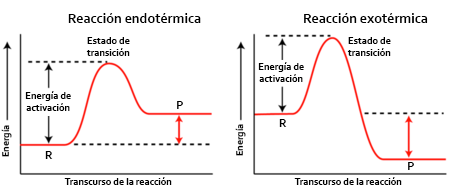
\includegraphics[width=0.8\textwidth]{Images/energia-activacion.png}
\end{figure}
